\documentclass[1p]{elsarticle_modified}
%\bibliographystyle{elsarticle-num}

%\usepackage[colorlinks]{hyperref}
%\usepackage{abbrmath_seonhwa} %\Abb, \Ascr, \Acal ,\Abf, \Afrak
\usepackage{amsfonts}
\usepackage{amssymb}
\usepackage{amsmath}
\usepackage{amsthm}
\usepackage{scalefnt}
\usepackage{amsbsy}
\usepackage{kotex}
\usepackage{caption}
\usepackage{subfig}
\usepackage{color}
\usepackage{graphicx}
\usepackage{xcolor} %% white, black, red, green, blue, cyan, magenta, yellow
\usepackage{float}
\usepackage{setspace}
\usepackage{hyperref}

\usepackage{tikz}
\usetikzlibrary{arrows}

\usepackage{multirow}
\usepackage{array} % fixed length table
\usepackage{hhline}

%%%%%%%%%%%%%%%%%%%%%
\makeatletter
\renewcommand*\env@matrix[1][\arraystretch]{%
	\edef\arraystretch{#1}%
	\hskip -\arraycolsep
	\let\@ifnextchar\new@ifnextchar
	\array{*\c@MaxMatrixCols c}}
\makeatother %https://tex.stackexchange.com/questions/14071/how-can-i-increase-the-line-spacing-in-a-matrix
%%%%%%%%%%%%%%%

\usepackage[normalem]{ulem}

\newcommand{\msout}[1]{\ifmmode\text{\sout{\ensuremath{#1}}}\else\sout{#1}\fi}
%SOURCE: \msout is \stkout macro in https://tex.stackexchange.com/questions/20609/strikeout-in-math-mode

\newcommand{\cancel}[1]{
	\ifmmode
	{\color{red}\msout{#1}}
	\else
	{\color{red}\sout{#1}}
	\fi
}

\newcommand{\add}[1]{
	{\color{blue}\uwave{#1}}
}

\newcommand{\replace}[2]{
	\ifmmode
	{\color{red}\msout{#1}}{\color{blue}\uwave{#2}}
	\else
	{\color{red}\sout{#1}}{\color{blue}\uwave{#2}}
	\fi
}

\newcommand{\Sol}{\mathcal{S}} %segment
\newcommand{\D}{D} %diagram
\newcommand{\A}{\mathcal{A}} %arc


%%%%%%%%%%%%%%%%%%%%%%%%%%%%%5 test

\def\sl{\operatorname{\textup{SL}}(2,\Cbb)}
\def\psl{\operatorname{\textup{PSL}}(2,\Cbb)}
\def\quan{\mkern 1mu \triangleright \mkern 1mu}

\theoremstyle{definition}
\newtheorem{thm}{Theorem}[section]
\newtheorem{prop}[thm]{Proposition}
\newtheorem{lem}[thm]{Lemma}
\newtheorem{ques}[thm]{Question}
\newtheorem{cor}[thm]{Corollary}
\newtheorem{defn}[thm]{Definition}
\newtheorem{exam}[thm]{Example}
\newtheorem{rmk}[thm]{Remark}
\newtheorem{alg}[thm]{Algorithm}

\newcommand{\I}{\sqrt{-1}}
\begin{document}

%\begin{frontmatter}
%
%\title{Boundary parabolic representations of knots up to 8 crossings}
%
%%% Group authors per affiliation:
%\author{Yunhi Cho} 
%\address{Department of Mathematics, University of Seoul, Seoul, Korea}
%\ead{yhcho@uos.ac.kr}
%
%
%\author{Seonhwa Kim} %\fnref{s_kim}}
%\address{Center for Geometry and Physics, Institute for Basic Science, Pohang, 37673, Korea}
%\ead{ryeona17@ibs.re.kr}
%
%\author{Hyuk Kim}
%\address{Department of Mathematical Sciences, Seoul National University, Seoul 08826, Korea}
%\ead{hyukkim@snu.ac.kr}
%
%\author{Seokbeom Yoon}
%\address{Department of Mathematical Sciences, Seoul National University, Seoul, 08826,  Korea}
%\ead{sbyoon15@snu.ac.kr}
%
%\begin{abstract}
%We find all boundary parabolic representation of knots up to 8 crossings.
%
%\end{abstract}
%\begin{keyword}
%    \MSC[2010] 57M25 
%\end{keyword}
%
%\end{frontmatter}

%\linenumbers
%\tableofcontents
%
\newcommand\colored[1]{\textcolor{white}{\rule[-0.35ex]{0.8em}{1.4ex}}\kern-0.8em\color{red} #1}%
%\newcommand\colored[1]{\textcolor{white}{ #1}\kern-2.17ex	\textcolor{white}{ #1}\kern-1.81ex	\textcolor{white}{ #1}\kern-2.15ex\color{red}#1	}

{\Large $\underline{12n_{0774}~(K12n_{0774})}$}

\setlength{\tabcolsep}{10pt}
\renewcommand{\arraystretch}{1.6}
\vspace{1cm}\begin{tabular}{m{100pt}>{\centering\arraybackslash}m{274pt}}
\multirow{5}{120pt}{
	\centering
	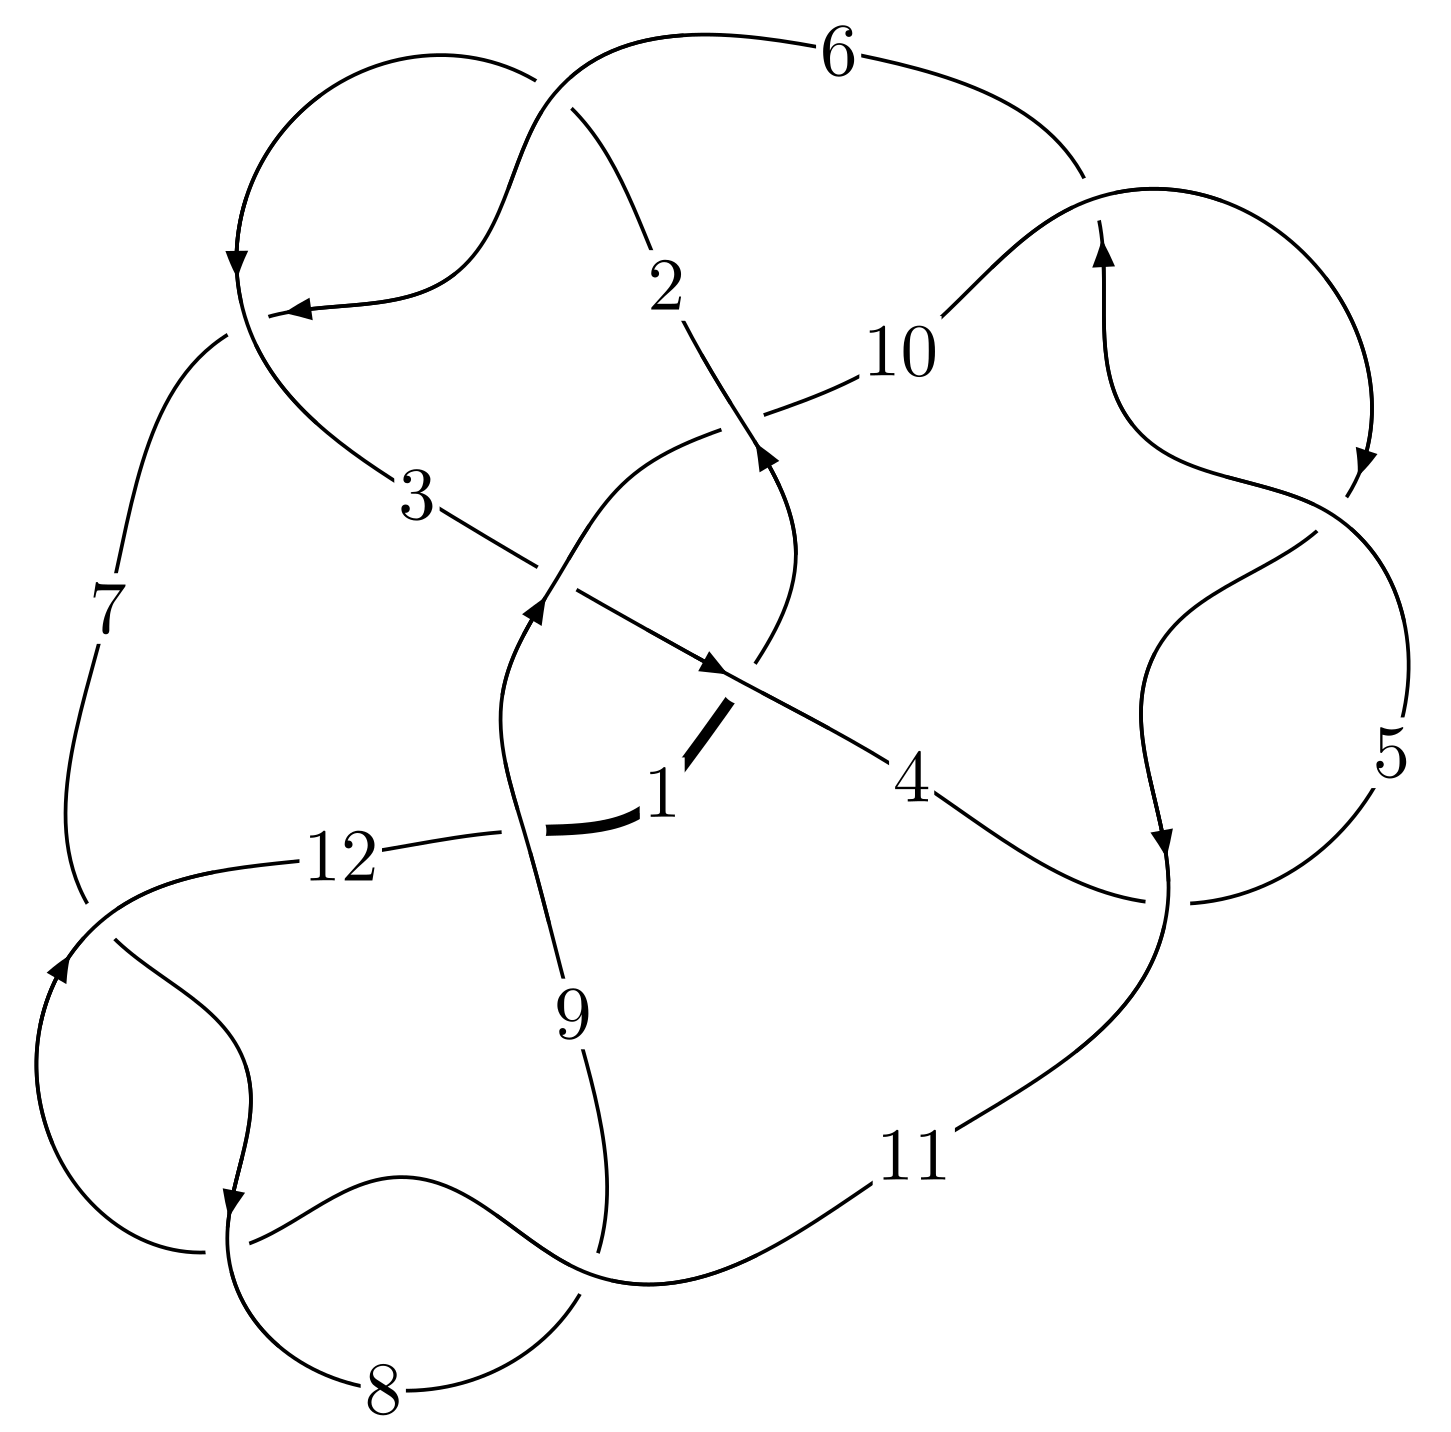
\includegraphics[width=112pt]{../../../GIT/diagram.site/Diagrams/png/2863_12n_0774.png}\\
\ \ \ A knot diagram\footnotemark}&
\allowdisplaybreaks
\textbf{Linearized knot diagam} \\
\cline{2-2}
 &
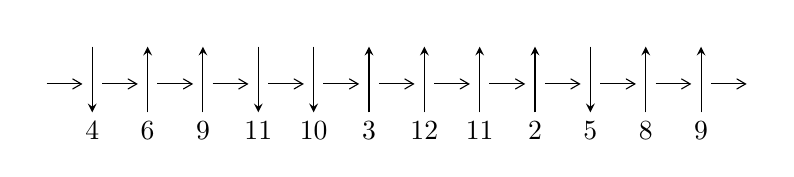
\begin{tikzpicture}[x=20pt, y=17pt]
	% nodes
	\node (C0) at (0, 0) {};
	\node (C1) at (1, 0) {};
	\node (C1U) at (1, +1) {};
	\node (C1D) at (1, -1) {4};

	\node (C2) at (2, 0) {};
	\node (C2U) at (2, +1) {};
	\node (C2D) at (2, -1) {6};

	\node (C3) at (3, 0) {};
	\node (C3U) at (3, +1) {};
	\node (C3D) at (3, -1) {9};

	\node (C4) at (4, 0) {};
	\node (C4U) at (4, +1) {};
	\node (C4D) at (4, -1) {11};

	\node (C5) at (5, 0) {};
	\node (C5U) at (5, +1) {};
	\node (C5D) at (5, -1) {10};

	\node (C6) at (6, 0) {};
	\node (C6U) at (6, +1) {};
	\node (C6D) at (6, -1) {3};

	\node (C7) at (7, 0) {};
	\node (C7U) at (7, +1) {};
	\node (C7D) at (7, -1) {12};

	\node (C8) at (8, 0) {};
	\node (C8U) at (8, +1) {};
	\node (C8D) at (8, -1) {11};

	\node (C9) at (9, 0) {};
	\node (C9U) at (9, +1) {};
	\node (C9D) at (9, -1) {2};

	\node (C10) at (10, 0) {};
	\node (C10U) at (10, +1) {};
	\node (C10D) at (10, -1) {5};

	\node (C11) at (11, 0) {};
	\node (C11U) at (11, +1) {};
	\node (C11D) at (11, -1) {8};

	\node (C12) at (12, 0) {};
	\node (C12U) at (12, +1) {};
	\node (C12D) at (12, -1) {9};
	\node (C13) at (13, 0) {};

	% arrows
	\draw[->,>={angle 60}]
	(C0) edge (C1) (C1) edge (C2) (C2) edge (C3) (C3) edge (C4) (C4) edge (C5) (C5) edge (C6) (C6) edge (C7) (C7) edge (C8) (C8) edge (C9) (C9) edge (C10) (C10) edge (C11) (C11) edge (C12) (C12) edge (C13) ;	\draw[->,>=stealth]
	(C1U) edge (C1D) (C2D) edge (C2U) (C3D) edge (C3U) (C4U) edge (C4D) (C5U) edge (C5D) (C6D) edge (C6U) (C7D) edge (C7U) (C8D) edge (C8U) (C9D) edge (C9U) (C10U) edge (C10D) (C11D) edge (C11U) (C12D) edge (C12U) ;
	\end{tikzpicture} \\
\hhline{~~} \\& 
\textbf{Solving Sequence} \\ \cline{2-2} 
 &
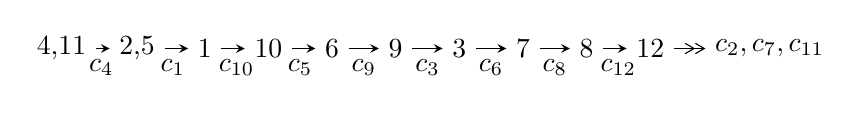
\begin{tikzpicture}[x=23pt, y=7pt]
	% node
	\node (A0) at (-1/8, 0) {4,11};
	\node (A1) at (17/16, 0) {2,5};
	\node (A2) at (17/8, 0) {1};
	\node (A3) at (25/8, 0) {10};
	\node (A4) at (33/8, 0) {6};
	\node (A5) at (41/8, 0) {9};
	\node (A6) at (49/8, 0) {3};
	\node (A7) at (57/8, 0) {7};
	\node (A8) at (65/8, 0) {8};
	\node (A9) at (73/8, 0) {12};
	\node (C1) at (1/2, -1) {$c_{4}$};
	\node (C2) at (13/8, -1) {$c_{1}$};
	\node (C3) at (21/8, -1) {$c_{10}$};
	\node (C4) at (29/8, -1) {$c_{5}$};
	\node (C5) at (37/8, -1) {$c_{9}$};
	\node (C6) at (45/8, -1) {$c_{3}$};
	\node (C7) at (53/8, -1) {$c_{6}$};
	\node (C8) at (61/8, -1) {$c_{8}$};
	\node (C9) at (69/8, -1) {$c_{12}$};
	\node (A10) at (11, 0) {$c_{2},c_{7},c_{11}$};

	% edge
	\draw[->,>=stealth]	
	(A0) edge (A1) (A1) edge (A2) (A2) edge (A3) (A3) edge (A4) (A4) edge (A5) (A5) edge (A6) (A6) edge (A7) (A7) edge (A8) (A8) edge (A9) ;
	\draw[->>,>={angle 60}]	
	(A9) edge (A10);
\end{tikzpicture} \\ 

\end{tabular} \\

\footnotetext{
The image of knot diagram is generated by the software ``\textbf{Draw programme}" developed by Andrew Bartholomew(\url{http://www.layer8.co.uk/maths/draw/index.htm\#Running-draw}), where we modified some parts for our purpose(\url{https://github.com/CATsTAILs/LinksPainter}).
}\phantom \\ \newline 
\centering \textbf{Ideals for irreducible components\footnotemark of $X_{\text{par}}$} 
 
\begin{align*}
I^u_{1}&=\langle 
6.62437\times10^{34} u^{37}-3.38900\times10^{34} u^{36}+\cdots+1.55713\times10^{36} b+2.95623\times10^{35},\\
\phantom{I^u_{1}}&\phantom{= \langle  }-1.51031\times10^{35} u^{37}-6.63829\times10^{35} u^{36}+\cdots+4.82710\times10^{37} a+1.02169\times10^{38},\\
\phantom{I^u_{1}}&\phantom{= \langle  }u^{38}- u^{37}+\cdots-43 u+31\rangle \\
I^u_{2}&=\langle 
- u^4-2 u^2+b,\;-2 u^9-12 u^7+u^6-26 u^5+6 u^4-25 u^3+10 u^2+a-11 u+4,\\
\phantom{I^u_{2}}&\phantom{= \langle  }u^{10}+6 u^8- u^7+13 u^6-5 u^5+13 u^4-8 u^3+7 u^2-4 u+1\rangle \\
I^u_{3}&=\langle 
b+u,\;a- u+1,\;u^3+2 u+1\rangle \\
\\
\end{align*}
\raggedright * 3 irreducible components of $\dim_{\mathbb{C}}=0$, with total 51 representations.\\
\footnotetext{All coefficients of polynomials are rational numbers. But the coefficients are sometimes approximated in decimal forms when there is not enough margin.}
\newpage
\renewcommand{\arraystretch}{1}
\centering \section*{I. $I^u_{1}= \langle 6.62\times10^{34} u^{37}-3.39\times10^{34} u^{36}+\cdots+1.56\times10^{36} b+2.96\times10^{35},\;-1.51\times10^{35} u^{37}-6.64\times10^{35} u^{36}+\cdots+4.83\times10^{37} a+1.02\times10^{38},\;u^{38}- u^{37}+\cdots-43 u+31 \rangle$}
\flushleft \textbf{(i) Arc colorings}\\
\begin{tabular}{m{7pt} m{180pt} m{7pt} m{180pt} }
\flushright $a_{4}=$&$\begin{pmatrix}1\\0\end{pmatrix}$ \\
\flushright $a_{11}=$&$\begin{pmatrix}0\\u\end{pmatrix}$ \\
\flushright $a_{2}=$&$\begin{pmatrix}0.00312880 u^{37}+0.0137521 u^{36}+\cdots-0.745993 u-2.11658\\-0.0425422 u^{37}+0.0217644 u^{36}+\cdots+0.229678 u-0.189851\end{pmatrix}$ \\
\flushright $a_{5}=$&$\begin{pmatrix}1\\u^2\end{pmatrix}$ \\
\flushright $a_{1}=$&$\begin{pmatrix}-0.0394133 u^{37}+0.0355165 u^{36}+\cdots-0.516316 u-2.30643\\-0.0425422 u^{37}+0.0217644 u^{36}+\cdots+0.229678 u-0.189851\end{pmatrix}$ \\
\flushright $a_{10}=$&$\begin{pmatrix}u\\u^3+u\end{pmatrix}$ \\
\flushright $a_{6}=$&$\begin{pmatrix}u^2+1\\u^4+2 u^2\end{pmatrix}$ \\
\flushright $a_{9}=$&$\begin{pmatrix}0.0349433 u^{37}-0.0282337 u^{36}+\cdots+3.18335 u-1.12201\\0.00748664 u^{37}-0.0301041 u^{36}+\cdots+1.94650 u-0.496751\end{pmatrix}$ \\
\flushright $a_{3}=$&$\begin{pmatrix}-0.0134487 u^{37}-0.0104237 u^{36}+\cdots+1.71946 u-0.562332\\-0.0504426 u^{37}+0.0543512 u^{36}+\cdots-0.337341 u+1.77353\end{pmatrix}$ \\
\flushright $a_{7}=$&$\begin{pmatrix}0.0100216 u^{37}-0.0217773 u^{36}+\cdots+2.92598 u-1.52154\\-0.0285363 u^{37}+0.118276 u^{36}+\cdots-1.14068 u-0.466351\end{pmatrix}$ \\
\flushright $a_{8}=$&$\begin{pmatrix}0.0349433 u^{37}-0.0282337 u^{36}+\cdots+3.18335 u-1.12201\\-0.0450590 u^{37}+0.00970789 u^{36}+\cdots+1.15176 u-0.704747\end{pmatrix}$ \\
\flushright $a_{12}=$&$\begin{pmatrix}0.0447886 u^{37}-0.00640128 u^{36}+\cdots-3.64544 u+0.609170\\-0.0494523 u^{37}+0.0164682 u^{36}+\cdots-0.878416 u-0.773098\end{pmatrix}$\\&\end{tabular}
\flushleft \textbf{(ii) Obstruction class $= -1$}\\~\\
\flushleft \textbf{(iii) Cusp Shapes $= 0.0331406 u^{37}+0.0412227 u^{36}+\cdots-15.9826 u-0.691715$}\\~\\
\newpage\renewcommand{\arraystretch}{1}
\flushleft \textbf{(iv) u-Polynomials at the component}\newline \\
\begin{tabular}{m{50pt}|m{274pt}}
Crossings & \hspace{64pt}u-Polynomials at each crossing \\
\hline $$\begin{aligned}c_{1}\end{aligned}$$&$\begin{aligned}
&u^{38}-5 u^{37}+\cdots-5335 u+599
\end{aligned}$\\
\hline $$\begin{aligned}c_{2},c_{6}\end{aligned}$$&$\begin{aligned}
&u^{38}-4 u^{37}+\cdots+538 u-98
\end{aligned}$\\
\hline $$\begin{aligned}c_{3}\end{aligned}$$&$\begin{aligned}
&u^{38}- u^{37}+\cdots-6836 u+799
\end{aligned}$\\
\hline $$\begin{aligned}c_{4},c_{5},c_{10}\end{aligned}$$&$\begin{aligned}
&u^{38}- u^{37}+\cdots-43 u+31
\end{aligned}$\\
\hline $$\begin{aligned}c_{7},c_{8},c_{11}\end{aligned}$$&$\begin{aligned}
&u^{38}+u^{37}+\cdots-33 u-1
\end{aligned}$\\
\hline $$\begin{aligned}c_{9}\end{aligned}$$&$\begin{aligned}
&u^{38}+2 u^{37}+\cdots+85 u-51
\end{aligned}$\\
\hline $$\begin{aligned}c_{12}\end{aligned}$$&$\begin{aligned}
&u^{38}- u^{37}+\cdots-7672 u-232
\end{aligned}$\\
\hline
\end{tabular}\\~\\
\newpage\renewcommand{\arraystretch}{1}
\flushleft \textbf{(v) Riley Polynomials at the component}\newline \\
\begin{tabular}{m{50pt}|m{274pt}}
Crossings & \hspace{64pt}Riley Polynomials at each crossing \\
\hline $$\begin{aligned}c_{1}\end{aligned}$$&$\begin{aligned}
&y^{38}-57 y^{37}+\cdots+6455881 y+358801
\end{aligned}$\\
\hline $$\begin{aligned}c_{2},c_{6}\end{aligned}$$&$\begin{aligned}
&y^{38}-18 y^{37}+\cdots-108928 y+9604
\end{aligned}$\\
\hline $$\begin{aligned}c_{3}\end{aligned}$$&$\begin{aligned}
&y^{38}+51 y^{37}+\cdots-5168514 y+638401
\end{aligned}$\\
\hline $$\begin{aligned}c_{4},c_{5},c_{10}\end{aligned}$$&$\begin{aligned}
&y^{38}+35 y^{37}+\cdots-1911 y+961
\end{aligned}$\\
\hline $$\begin{aligned}c_{7},c_{8},c_{11}\end{aligned}$$&$\begin{aligned}
&y^{38}+53 y^{37}+\cdots-1289 y+1
\end{aligned}$\\
\hline $$\begin{aligned}c_{9}\end{aligned}$$&$\begin{aligned}
&y^{38}-18 y^{37}+\cdots-30685 y+2601
\end{aligned}$\\
\hline $$\begin{aligned}c_{12}\end{aligned}$$&$\begin{aligned}
&y^{38}+137 y^{37}+\cdots-68527952 y+53824
\end{aligned}$\\
\hline
\end{tabular}\\~\\
\newpage\flushleft \textbf{(vi) Complex Volumes and Cusp Shapes}
$$\begin{array}{c|c|c}  
\text{Solutions to }I^u_{1}& \I (\text{vol} + \sqrt{-1}CS) & \text{Cusp shape}\\
 \hline 
\begin{aligned}
u &= -0.638019 + 0.750388 I \\
a &= -0.0267617 + 0.1147200 I \\
b &= \phantom{-}0.722696 + 0.604621 I\end{aligned}
 & \phantom{-}0.0307983 + 0.0668754 I & \phantom{-}5.97468 + 0.20302 I \\ \hline\begin{aligned}
u &= -0.638019 - 0.750388 I \\
a &= -0.0267617 - 0.1147200 I \\
b &= \phantom{-}0.722696 - 0.604621 I\end{aligned}
 & \phantom{-}0.0307983 - 0.0668754 I & \phantom{-}5.97468 - 0.20302 I \\ \hline\begin{aligned}
u &= -0.205648 + 1.005780 I \\
a &= -1.065570 + 0.155067 I \\
b &= \phantom{-}0.566243 - 0.700302 I\end{aligned}
 & \phantom{-}0.30073 + 3.12728 I & \phantom{-}5.74339 - 3.05475 I \\ \hline\begin{aligned}
u &= -0.205648 - 1.005780 I \\
a &= -1.065570 - 0.155067 I \\
b &= \phantom{-}0.566243 + 0.700302 I\end{aligned}
 & \phantom{-}0.30073 - 3.12728 I & \phantom{-}5.74339 + 3.05475 I \\ \hline\begin{aligned}
u &= -0.808673 + 0.138234 I \\
a &= \phantom{-}1.29598 + 0.61262 I \\
b &= \phantom{-}1.050550 - 0.092879 I\end{aligned}
 & -1.57428 + 4.12934 I & \phantom{-}1.75204 - 5.88893 I \\ \hline\begin{aligned}
u &= -0.808673 - 0.138234 I \\
a &= \phantom{-}1.29598 - 0.61262 I \\
b &= \phantom{-}1.050550 + 0.092879 I\end{aligned}
 & -1.57428 - 4.12934 I & \phantom{-}1.75204 + 5.88893 I \\ \hline\begin{aligned}
u &= \phantom{-}0.186789 + 1.179420 I \\
a &= \phantom{-}0.437334 + 0.307728 I \\
b &= -1.43772 + 0.15241 I\end{aligned}
 & -0.62020 - 1.71292 I & \phantom{-}7.11578 + 4.48405 I \\ \hline\begin{aligned}
u &= \phantom{-}0.186789 - 1.179420 I \\
a &= \phantom{-}0.437334 - 0.307728 I \\
b &= -1.43772 - 0.15241 I\end{aligned}
 & -0.62020 + 1.71292 I & \phantom{-}7.11578 - 4.48405 I \\ \hline\begin{aligned}
u &= -0.035830 + 1.196030 I \\
a &= \phantom{-}0.74364 + 1.35480 I \\
b &= -0.094716 + 0.338801 I\end{aligned}
 & \phantom{-}1.54048 - 1.51605 I & \phantom{-}5.47077 + 1.56313 I \\ \hline\begin{aligned}
u &= -0.035830 - 1.196030 I \\
a &= \phantom{-}0.74364 - 1.35480 I \\
b &= -0.094716 - 0.338801 I\end{aligned}
 & \phantom{-}1.54048 + 1.51605 I & \phantom{-}5.47077 - 1.56313 I\\
 \hline 
 \end{array}$$\newpage$$\begin{array}{c|c|c}  
\text{Solutions to }I^u_{1}& \I (\text{vol} + \sqrt{-1}CS) & \text{Cusp shape}\\
 \hline 
\begin{aligned}
u &= \phantom{-}1.191440 + 0.333174 I \\
a &= \phantom{-}1.043410 - 0.369661 I \\
b &= \phantom{-}2.01038 + 0.71201 I\end{aligned}
 & -12.06790 - 6.30873 I & \phantom{-}2.13106 + 4.45047 I \\ \hline\begin{aligned}
u &= \phantom{-}1.191440 - 0.333174 I \\
a &= \phantom{-}1.043410 + 0.369661 I \\
b &= \phantom{-}2.01038 - 0.71201 I\end{aligned}
 & -12.06790 + 6.30873 I & \phantom{-}2.13106 - 4.45047 I \\ \hline\begin{aligned}
u &= -0.728989 + 0.094813 I \\
a &= -2.26028 + 0.66699 I \\
b &= -2.27756 + 0.23999 I\end{aligned}
 & -13.44440 + 0.57800 I & \phantom{-}0.020927 + 0.338279 I \\ \hline\begin{aligned}
u &= -0.728989 - 0.094813 I \\
a &= -2.26028 - 0.66699 I \\
b &= -2.27756 - 0.23999 I\end{aligned}
 & -13.44440 - 0.57800 I & \phantom{-}0.020927 - 0.338279 I \\ \hline\begin{aligned}
u &= \phantom{-}0.270004 + 1.252220 I \\
a &= \phantom{-}0.282766 - 1.337250 I \\
b &= \phantom{-}0.757575 - 0.249175 I\end{aligned}
 & \phantom{-}5.78248 - 3.21327 I & \phantom{-}7.91783 + 2.84424 I \\ \hline\begin{aligned}
u &= \phantom{-}0.270004 - 1.252220 I \\
a &= \phantom{-}0.282766 + 1.337250 I \\
b &= \phantom{-}0.757575 + 0.249175 I\end{aligned}
 & \phantom{-}5.78248 + 3.21327 I & \phantom{-}7.91783 - 2.84424 I \\ \hline\begin{aligned}
u &= -0.328477 + 1.291160 I \\
a &= \phantom{-}1.19013 - 2.17034 I \\
b &= -2.48972 - 0.49981 I\end{aligned}
 & -9.66385 + 3.20076 I & \phantom{-}5.89501 - 3.23003 I \\ \hline\begin{aligned}
u &= -0.328477 - 1.291160 I \\
a &= \phantom{-}1.19013 + 2.17034 I \\
b &= -2.48972 + 0.49981 I\end{aligned}
 & -9.66385 - 3.20076 I & \phantom{-}5.89501 + 3.23003 I \\ \hline\begin{aligned}
u &= \phantom{-}0.615140\phantom{ +0.000000I} \\
a &= \phantom{-}1.71995\phantom{ +0.000000I} \\
b &= \phantom{-}0.634685\phantom{ +0.000000I}\end{aligned}
 & \phantom{-}1.97433\phantom{ +0.000000I} & \phantom{-}3.38590\phantom{ +0.000000I} \\ \hline\begin{aligned}
u &= -0.198749 + 0.555559 I \\
a &= \phantom{-}0.466569 - 0.230649 I \\
b &= -0.042075 + 0.321375 I\end{aligned}
 & \phantom{-}0.293656 + 0.891269 I & \phantom{-}6.04844 - 7.62734 I\\
 \hline 
 \end{array}$$\newpage$$\begin{array}{c|c|c}  
\text{Solutions to }I^u_{1}& \I (\text{vol} + \sqrt{-1}CS) & \text{Cusp shape}\\
 \hline 
\begin{aligned}
u &= -0.198749 - 0.555559 I \\
a &= \phantom{-}0.466569 + 0.230649 I \\
b &= -0.042075 - 0.321375 I\end{aligned}
 & \phantom{-}0.293656 - 0.891269 I & \phantom{-}6.04844 + 7.62734 I \\ \hline\begin{aligned}
u &= \phantom{-}0.19095 + 1.40255 I \\
a &= -0.762581 + 0.804443 I \\
b &= \phantom{-}0.648853 - 0.396327 I\end{aligned}
 & \phantom{-}7.52810 - 2.72251 I & \phantom{-}5.91943 + 2.93635 I \\ \hline\begin{aligned}
u &= \phantom{-}0.19095 - 1.40255 I \\
a &= -0.762581 - 0.804443 I \\
b &= \phantom{-}0.648853 + 0.396327 I\end{aligned}
 & \phantom{-}7.52810 + 2.72251 I & \phantom{-}5.91943 - 2.93635 I \\ \hline\begin{aligned}
u &= -0.33162 + 1.39639 I \\
a &= \phantom{-}0.384147 - 0.722282 I \\
b &= -2.04211 + 0.03629 I\end{aligned}
 & -8.62803 + 4.45679 I & \phantom{-}4.27715 - 2.52282 I \\ \hline\begin{aligned}
u &= -0.33162 - 1.39639 I \\
a &= \phantom{-}0.384147 + 0.722282 I \\
b &= -2.04211 - 0.03629 I\end{aligned}
 & -8.62803 - 4.45679 I & \phantom{-}4.27715 + 2.52282 I \\ \hline\begin{aligned}
u &= \phantom{-}0.560762\phantom{ +0.000000I} \\
a &= -0.627330\phantom{ +0.000000I} \\
b &= \phantom{-}0.630030\phantom{ +0.000000I}\end{aligned}
 & \phantom{-}2.83334\phantom{ +0.000000I} & -3.70100\phantom{ +0.000000I} \\ \hline\begin{aligned}
u &= -0.39837 + 1.38695 I \\
a &= -0.00124 + 1.46170 I \\
b &= \phantom{-}1.46915 - 0.06976 I\end{aligned}
 & \phantom{-}3.24411 + 8.61128 I & \phantom{-}5.93302 - 6.50406 I \\ \hline\begin{aligned}
u &= -0.39837 - 1.38695 I \\
a &= -0.00124 - 1.46170 I \\
b &= \phantom{-}1.46915 + 0.06976 I\end{aligned}
 & \phantom{-}3.24411 - 8.61128 I & \phantom{-}5.93302 + 6.50406 I \\ \hline\begin{aligned}
u &= \phantom{-}0.456864 + 0.208287 I \\
a &= -0.90969 + 1.40386 I \\
b &= -1.084480 - 0.415889 I\end{aligned}
 & -3.49555 - 0.69535 I & -2.34683 + 1.44862 I \\ \hline\begin{aligned}
u &= \phantom{-}0.456864 - 0.208287 I \\
a &= -0.90969 - 1.40386 I \\
b &= -1.084480 + 0.415889 I\end{aligned}
 & -3.49555 + 0.69535 I & -2.34683 - 1.44862 I\\
 \hline 
 \end{array}$$\newpage$$\begin{array}{c|c|c}  
\text{Solutions to }I^u_{1}& \I (\text{vol} + \sqrt{-1}CS) & \text{Cusp shape}\\
 \hline 
\begin{aligned}
u &= \phantom{-}0.87973 + 1.22637 I \\
a &= -0.139604 - 0.532893 I \\
b &= \phantom{-}1.63216 - 0.82120 I\end{aligned}
 & -9.52612 - 0.81474 I & \phantom{-}4.00000 + 0. I\phantom{ +0.000000I} \\ \hline\begin{aligned}
u &= \phantom{-}0.87973 - 1.22637 I \\
a &= -0.139604 + 0.532893 I \\
b &= \phantom{-}1.63216 + 0.82120 I\end{aligned}
 & -9.52612 + 0.81474 I & \phantom{-}4.00000 + 0. I\phantom{ +0.000000I} \\ \hline\begin{aligned}
u &= \phantom{-}0.05021 + 1.52644 I \\
a &= \phantom{-}0.17157 + 1.59718 I \\
b &= -0.18166 - 1.41300 I\end{aligned}
 & \phantom{-}2.16967 - 2.20129 I & \phantom{-}4.00000 + 3.06497 I \\ \hline\begin{aligned}
u &= \phantom{-}0.05021 - 1.52644 I \\
a &= \phantom{-}0.17157 - 1.59718 I \\
b &= -0.18166 + 1.41300 I\end{aligned}
 & \phantom{-}2.16967 + 2.20129 I & \phantom{-}4.00000 - 3.06497 I \\ \hline\begin{aligned}
u &= -0.12317 + 1.58705 I \\
a &= -0.40122 - 1.36947 I \\
b &= \phantom{-}0.37780 + 1.57073 I\end{aligned}
 & \phantom{-}8.12130 + 2.40437 I & \phantom{-}4.00000 + 0. I\phantom{ +0.000000I} \\ \hline\begin{aligned}
u &= -0.12317 - 1.58705 I \\
a &= -0.40122 + 1.36947 I \\
b &= \phantom{-}0.37780 - 1.57073 I\end{aligned}
 & \phantom{-}8.12130 - 2.40437 I & \phantom{-}4.00000 + 0. I\phantom{ +0.000000I} \\ \hline\begin{aligned}
u &= \phantom{-}0.48360 + 1.54293 I \\
a &= -0.14007 - 1.57905 I \\
b &= \phantom{-}2.28229 + 0.66578 I\end{aligned}
 & -6.11597 - 12.29010 I & \phantom{-0.000000 } 0 \\ \hline\begin{aligned}
u &= \phantom{-}0.48360 - 1.54293 I \\
a &= -0.14007 + 1.57905 I \\
b &= \phantom{-}2.28229 - 0.66578 I\end{aligned}
 & -6.11597 + 12.29010 I & \phantom{-0.000000 } 0\\
 \hline 
 \end{array}$$\newpage\newpage\renewcommand{\arraystretch}{1}
\centering \section*{II. $I^u_{2}= \langle - u^4-2 u^2+b,\;-2 u^9-12 u^7+\cdots+a+4,\;u^{10}+6 u^8+\cdots-4 u+1 \rangle$}
\flushleft \textbf{(i) Arc colorings}\\
\begin{tabular}{m{7pt} m{180pt} m{7pt} m{180pt} }
\flushright $a_{4}=$&$\begin{pmatrix}1\\0\end{pmatrix}$ \\
\flushright $a_{11}=$&$\begin{pmatrix}0\\u\end{pmatrix}$ \\
\flushright $a_{2}=$&$\begin{pmatrix}2 u^9+12 u^7- u^6+26 u^5-6 u^4+25 u^3-10 u^2+11 u-4\\u^4+2 u^2\end{pmatrix}$ \\
\flushright $a_{5}=$&$\begin{pmatrix}1\\u^2\end{pmatrix}$ \\
\flushright $a_{1}=$&$\begin{pmatrix}2 u^9+12 u^7- u^6+26 u^5-5 u^4+25 u^3-8 u^2+11 u-4\\u^4+2 u^2\end{pmatrix}$ \\
\flushright $a_{10}=$&$\begin{pmatrix}u\\u^3+u\end{pmatrix}$ \\
\flushright $a_{6}=$&$\begin{pmatrix}u^2+1\\u^4+2 u^2\end{pmatrix}$ \\
\flushright $a_{9}=$&$\begin{pmatrix}2 u^9+u^8+12 u^7+4 u^6+25 u^5+3 u^4+22 u^3-3 u^2+9 u-2\\u^3+2 u\end{pmatrix}$ \\
\flushright $a_{3}=$&$\begin{pmatrix}2 u^9+12 u^7- u^6+26 u^5-5 u^4+25 u^3-8 u^2+11 u-3\\u^6+4 u^4+4 u^2\end{pmatrix}$ \\
\flushright $a_{7}=$&$\begin{pmatrix}-2 u^9- u^8-12 u^7-4 u^6-25 u^5-3 u^4-22 u^3+4 u^2-9 u+4\\- u^8-5 u^6-7 u^4-2 u^2\end{pmatrix}$ \\
\flushright $a_{8}=$&$\begin{pmatrix}2 u^9+u^8+12 u^7+4 u^6+25 u^5+3 u^4+22 u^3-3 u^2+9 u-2\\u^5+4 u^3- u^2+4 u-1\end{pmatrix}$ \\
\flushright $a_{12}=$&$\begin{pmatrix}u^9+6 u^7- u^6+13 u^5-6 u^4+13 u^3-11 u^2+7 u-6\\u^7- u^6+5 u^5-4 u^4+8 u^3-5 u^2+4 u-2\end{pmatrix}$\\&\end{tabular}
\flushleft \textbf{(ii) Obstruction class $= 1$}\\~\\
\flushleft \textbf{(iii) Cusp Shapes $= -2 u^8+3 u^7-8 u^6+13 u^5-11 u^4+19 u^3-11 u^2+11 u-2$}\\~\\
\newpage\renewcommand{\arraystretch}{1}
\flushleft \textbf{(iv) u-Polynomials at the component}\newline \\
\begin{tabular}{m{50pt}|m{274pt}}
Crossings & \hspace{64pt}u-Polynomials at each crossing \\
\hline $$\begin{aligned}c_{1}\end{aligned}$$&$\begin{aligned}
&u^{10}-4 u^9+4 u^8-3 u^7+11 u^6-7 u^5- u^4-8 u^3+5 u^2+2 u+1
\end{aligned}$\\
\hline $$\begin{aligned}c_{2}\end{aligned}$$&$\begin{aligned}
&u^{10}-2 u^9- u^8+3 u^7+2 u^5-2 u^4-5 u^3+2 u^2+2 u+1
\end{aligned}$\\
\hline $$\begin{aligned}c_{3}\end{aligned}$$&$\begin{aligned}
&u^{10}-3 u^9+8 u^8-12 u^7+13 u^6-11 u^5+6 u^4- u^3+u^2-2 u+1
\end{aligned}$\\
\hline $$\begin{aligned}c_{4},c_{5}\end{aligned}$$&$\begin{aligned}
&u^{10}+6 u^8- u^7+13 u^6-5 u^5+13 u^4-8 u^3+7 u^2-4 u+1
\end{aligned}$\\
\hline $$\begin{aligned}c_{6}\end{aligned}$$&$\begin{aligned}
&u^{10}+2 u^9- u^8-3 u^7-2 u^5-2 u^4+5 u^3+2 u^2-2 u+1
\end{aligned}$\\
\hline $$\begin{aligned}c_{7},c_{8}\end{aligned}$$&$\begin{aligned}
&u^{10}+7 u^8- u^7+17 u^6-5 u^5+17 u^4-8 u^3+6 u^2-4 u+1
\end{aligned}$\\
\hline $$\begin{aligned}c_{9}\end{aligned}$$&$\begin{aligned}
&u^{10}-2 u^9+u^8- u^7+6 u^6-11 u^5+13 u^4-12 u^3+8 u^2-3 u+1
\end{aligned}$\\
\hline $$\begin{aligned}c_{10}\end{aligned}$$&$\begin{aligned}
&u^{10}+6 u^8+u^7+13 u^6+5 u^5+13 u^4+8 u^3+7 u^2+4 u+1
\end{aligned}$\\
\hline $$\begin{aligned}c_{11}\end{aligned}$$&$\begin{aligned}
&u^{10}+7 u^8+u^7+17 u^6+5 u^5+17 u^4+8 u^3+6 u^2+4 u+1
\end{aligned}$\\
\hline $$\begin{aligned}c_{12}\end{aligned}$$&$\begin{aligned}
&u^{10}+3 u^9+\cdots+6 u+1
\end{aligned}$\\
\hline
\end{tabular}\\~\\
\newpage\renewcommand{\arraystretch}{1}
\flushleft \textbf{(v) Riley Polynomials at the component}\newline \\
\begin{tabular}{m{50pt}|m{274pt}}
Crossings & \hspace{64pt}Riley Polynomials at each crossing \\
\hline $$\begin{aligned}c_{1}\end{aligned}$$&$\begin{aligned}
&y^{10}-8 y^9+\cdots+6 y+1
\end{aligned}$\\
\hline $$\begin{aligned}c_{2},c_{6}\end{aligned}$$&$\begin{aligned}
&y^{10}-6 y^9+13 y^8-5 y^7-24 y^6+32 y^5+10 y^4-41 y^3+20 y^2+1
\end{aligned}$\\
\hline $$\begin{aligned}c_{3}\end{aligned}$$&$\begin{aligned}
&y^{10}+7 y^9+18 y^8+10 y^7-3 y^6+17 y^5+8 y^4-7 y^3+9 y^2-2 y+1
\end{aligned}$\\
\hline $$\begin{aligned}c_{4},c_{5},c_{10}\end{aligned}$$&$\begin{aligned}
&y^{10}+12 y^9+\cdots-2 y+1
\end{aligned}$\\
\hline $$\begin{aligned}c_{7},c_{8},c_{11}\end{aligned}$$&$\begin{aligned}
&y^{10}+14 y^9+\cdots-4 y+1
\end{aligned}$\\
\hline $$\begin{aligned}c_{9}\end{aligned}$$&$\begin{aligned}
&y^{10}-2 y^9+9 y^8-7 y^7+8 y^6+17 y^5-3 y^4+10 y^3+18 y^2+7 y+1
\end{aligned}$\\
\hline $$\begin{aligned}c_{12}\end{aligned}$$&$\begin{aligned}
&y^{10}+25 y^9+\cdots+2 y+1
\end{aligned}$\\
\hline
\end{tabular}\\~\\
\newpage\flushleft \textbf{(vi) Complex Volumes and Cusp Shapes}
$$\begin{array}{c|c|c}  
\text{Solutions to }I^u_{2}& \I (\text{vol} + \sqrt{-1}CS) & \text{Cusp shape}\\
 \hline 
\begin{aligned}
u &= \phantom{-}0.203188 + 0.867061 I \\
a &= \phantom{-}0.493495 + 0.731043 I \\
b &= -1.040350 + 0.204005 I\end{aligned}
 & -1.57782 - 0.69065 I & \phantom{-}1.59727 + 0.69033 I \\ \hline\begin{aligned}
u &= \phantom{-}0.203188 - 0.867061 I \\
a &= \phantom{-}0.493495 - 0.731043 I \\
b &= -1.040350 - 0.204005 I\end{aligned}
 & -1.57782 + 0.69065 I & \phantom{-}1.59727 - 0.69033 I \\ \hline\begin{aligned}
u &= -0.518951 + 1.046120 I \\
a &= \phantom{-}0.16725 - 1.58982 I \\
b &= -2.14828 - 0.37991 I\end{aligned}
 & -10.93840 + 1.99907 I & \phantom{-}1.90479 - 0.88974 I \\ \hline\begin{aligned}
u &= -0.518951 - 1.046120 I \\
a &= \phantom{-}0.16725 + 1.58982 I \\
b &= -2.14828 + 0.37991 I\end{aligned}
 & -10.93840 - 1.99907 I & \phantom{-}1.90479 + 0.88974 I \\ \hline\begin{aligned}
u &= \phantom{-}0.09726 + 1.51614 I \\
a &= -0.226826 + 1.186790 I \\
b &= \phantom{-}0.575141 - 0.760414 I\end{aligned}
 & \phantom{-}4.87853 - 4.08278 I & \phantom{-}5.39048 + 3.19814 I \\ \hline\begin{aligned}
u &= \phantom{-}0.09726 - 1.51614 I \\
a &= -0.226826 - 1.186790 I \\
b &= \phantom{-}0.575141 + 0.760414 I\end{aligned}
 & \phantom{-}4.87853 + 4.08278 I & \phantom{-}5.39048 - 3.19814 I \\ \hline\begin{aligned}
u &= -0.15182 + 1.51661 I \\
a &= -0.58645 - 1.30038 I \\
b &= \phantom{-}0.418801 + 1.176140 I\end{aligned}
 & \phantom{-}8.85979 + 2.29290 I & \phantom{-}14.4139 - 0.8018 I \\ \hline\begin{aligned}
u &= -0.15182 - 1.51661 I \\
a &= -0.58645 + 1.30038 I \\
b &= \phantom{-}0.418801 - 1.176140 I\end{aligned}
 & \phantom{-}8.85979 - 2.29290 I & \phantom{-}14.4139 + 0.8018 I \\ \hline\begin{aligned}
u &= \phantom{-}0.370323 + 0.187881 I \\
a &= -0.84746 + 2.49473 I \\
b &= \phantom{-}0.194686 + 0.306649 I\end{aligned}
 & -1.22208 - 2.50161 I & \phantom{-}1.19353 + 1.66838 I \\ \hline\begin{aligned}
u &= \phantom{-}0.370323 - 0.187881 I \\
a &= -0.84746 - 2.49473 I \\
b &= \phantom{-}0.194686 - 0.306649 I\end{aligned}
 & -1.22208 + 2.50161 I & \phantom{-}1.19353 - 1.66838 I\\
 \hline 
 \end{array}$$\newpage\newpage\renewcommand{\arraystretch}{1}
\centering \section*{III. $I^u_{3}= \langle b+u,\;a- u+1,\;u^3+2 u+1 \rangle$}
\flushleft \textbf{(i) Arc colorings}\\
\begin{tabular}{m{7pt} m{180pt} m{7pt} m{180pt} }
\flushright $a_{4}=$&$\begin{pmatrix}1\\0\end{pmatrix}$ \\
\flushright $a_{11}=$&$\begin{pmatrix}0\\u\end{pmatrix}$ \\
\flushright $a_{2}=$&$\begin{pmatrix}u-1\\- u\end{pmatrix}$ \\
\flushright $a_{5}=$&$\begin{pmatrix}1\\u^2\end{pmatrix}$ \\
\flushright $a_{1}=$&$\begin{pmatrix}-1\\- u\end{pmatrix}$ \\
\flushright $a_{10}=$&$\begin{pmatrix}u\\- u-1\end{pmatrix}$ \\
\flushright $a_{6}=$&$\begin{pmatrix}u^2+1\\- u\end{pmatrix}$ \\
\flushright $a_{9}=$&$\begin{pmatrix}1\\-1\end{pmatrix}$ \\
\flushright $a_{3}=$&$\begin{pmatrix}0\\1\end{pmatrix}$ \\
\flushright $a_{7}=$&$\begin{pmatrix}u^2+1\\- u^2- u-1\end{pmatrix}$ \\
\flushright $a_{8}=$&$\begin{pmatrix}1\\u^2-1\end{pmatrix}$ \\
\flushright $a_{12}=$&$\begin{pmatrix}u\\-2 u-1\end{pmatrix}$\\&\end{tabular}
\flushleft \textbf{(ii) Obstruction class $= 1$}\\~\\
\flushleft \textbf{(iii) Cusp Shapes $= 3 u^2- u+14$}\\~\\
\newpage\renewcommand{\arraystretch}{1}
\flushleft \textbf{(iv) u-Polynomials at the component}\newline \\
\begin{tabular}{m{50pt}|m{274pt}}
Crossings & \hspace{64pt}u-Polynomials at each crossing \\
\hline $$\begin{aligned}c_{1},c_{4},c_{5}\\c_{7},c_{8}\end{aligned}$$&$\begin{aligned}
&u^3+2 u+1
\end{aligned}$\\
\hline $$\begin{aligned}c_{2}\end{aligned}$$&$\begin{aligned}
&u^3- u^2- u+2
\end{aligned}$\\
\hline $$\begin{aligned}c_{3},c_{9}\end{aligned}$$&$\begin{aligned}
&(u+1)^3
\end{aligned}$\\
\hline $$\begin{aligned}c_{6}\end{aligned}$$&$\begin{aligned}
&u^3+u^2- u-2
\end{aligned}$\\
\hline $$\begin{aligned}c_{10},c_{11}\end{aligned}$$&$\begin{aligned}
&u^3+2 u-1
\end{aligned}$\\
\hline $$\begin{aligned}c_{12}\end{aligned}$$&$\begin{aligned}
&u^3-3 u^2+5 u-2
\end{aligned}$\\
\hline
\end{tabular}\\~\\
\newpage\renewcommand{\arraystretch}{1}
\flushleft \textbf{(v) Riley Polynomials at the component}\newline \\
\begin{tabular}{m{50pt}|m{274pt}}
Crossings & \hspace{64pt}Riley Polynomials at each crossing \\
\hline $$\begin{aligned}c_{1},c_{4},c_{5}\\c_{7},c_{8},c_{10}\\c_{11}\end{aligned}$$&$\begin{aligned}
&y^3+4 y^2+4 y-1
\end{aligned}$\\
\hline $$\begin{aligned}c_{2},c_{6}\end{aligned}$$&$\begin{aligned}
&y^3-3 y^2+5 y-4
\end{aligned}$\\
\hline $$\begin{aligned}c_{3},c_{9}\end{aligned}$$&$\begin{aligned}
&(y-1)^3
\end{aligned}$\\
\hline $$\begin{aligned}c_{12}\end{aligned}$$&$\begin{aligned}
&y^3+y^2+13 y-4
\end{aligned}$\\
\hline
\end{tabular}\\~\\
\newpage\flushleft \textbf{(vi) Complex Volumes and Cusp Shapes}
$$\begin{array}{c|c|c}  
\text{Solutions to }I^u_{3}& \I (\text{vol} + \sqrt{-1}CS) & \text{Cusp shape}\\
 \hline 
\begin{aligned}
u &= \phantom{-}0.22670 + 1.46771 I \\
a &= -0.77330 + 1.46771 I \\
b &= -0.22670 - 1.46771 I\end{aligned}
 & \phantom{-}3.28987\phantom{ +0.000000I} & \phantom{-}7.46495 + 0.52866 I \\ \hline\begin{aligned}
u &= \phantom{-}0.22670 - 1.46771 I \\
a &= -0.77330 - 1.46771 I \\
b &= -0.22670 + 1.46771 I\end{aligned}
 & \phantom{-}3.28987\phantom{ +0.000000I} & \phantom{-}7.46495 - 0.52866 I \\ \hline\begin{aligned}
u &= -0.453398\phantom{ +0.000000I} \\
a &= -1.45340\phantom{ +0.000000I} \\
b &= \phantom{-}0.453398\phantom{ +0.000000I}\end{aligned}
 & \phantom{-}3.28987\phantom{ +0.000000I} & \phantom{-}15.0700\phantom{ +0.000000I}\\
 \hline 
 \end{array}$$\newpage
\newpage\renewcommand{\arraystretch}{1}
\centering \section*{ IV. u-Polynomials}
\begin{tabular}{m{50pt}|m{274pt}}
Crossings & \hspace{64pt}u-Polynomials at each crossing \\
\hline $$\begin{aligned}c_{1}\end{aligned}$$&$\begin{aligned}
&(u^3+2 u+1)\\
&\cdot(u^{10}-4 u^9+4 u^8-3 u^7+11 u^6-7 u^5- u^4-8 u^3+5 u^2+2 u+1)\\
&\cdot(u^{38}-5 u^{37}+\cdots-5335 u+599)
\end{aligned}$\\
\hline $$\begin{aligned}c_{2}\end{aligned}$$&$\begin{aligned}
&(u^3- u^2- u+2)(u^{10}-2 u^9+\cdots+2 u+1)\\
&\cdot(u^{38}-4 u^{37}+\cdots+538 u-98)
\end{aligned}$\\
\hline $$\begin{aligned}c_{3}\end{aligned}$$&$\begin{aligned}
&(u+1)^3\\
&\cdot(u^{10}-3 u^9+8 u^8-12 u^7+13 u^6-11 u^5+6 u^4- u^3+u^2-2 u+1)\\
&\cdot(u^{38}- u^{37}+\cdots-6836 u+799)
\end{aligned}$\\
\hline $$\begin{aligned}c_{4},c_{5}\end{aligned}$$&$\begin{aligned}
&(u^3+2 u+1)(u^{10}+6 u^8+\cdots-4 u+1)\\
&\cdot(u^{38}- u^{37}+\cdots-43 u+31)
\end{aligned}$\\
\hline $$\begin{aligned}c_{6}\end{aligned}$$&$\begin{aligned}
&(u^3+u^2- u-2)(u^{10}+2 u^9+\cdots-2 u+1)\\
&\cdot(u^{38}-4 u^{37}+\cdots+538 u-98)
\end{aligned}$\\
\hline $$\begin{aligned}c_{7},c_{8}\end{aligned}$$&$\begin{aligned}
&(u^3+2 u+1)(u^{10}+7 u^8+\cdots-4 u+1)\\
&\cdot(u^{38}+u^{37}+\cdots-33 u-1)
\end{aligned}$\\
\hline $$\begin{aligned}c_{9}\end{aligned}$$&$\begin{aligned}
&(u+1)^3\\
&\cdot(u^{10}-2 u^9+u^8- u^7+6 u^6-11 u^5+13 u^4-12 u^3+8 u^2-3 u+1)\\
&\cdot(u^{38}+2 u^{37}+\cdots+85 u-51)
\end{aligned}$\\
\hline $$\begin{aligned}c_{10}\end{aligned}$$&$\begin{aligned}
&(u^3+2 u-1)(u^{10}+6 u^8+\cdots+4 u+1)\\
&\cdot(u^{38}- u^{37}+\cdots-43 u+31)
\end{aligned}$\\
\hline $$\begin{aligned}c_{11}\end{aligned}$$&$\begin{aligned}
&(u^3+2 u-1)(u^{10}+7 u^8+\cdots+4 u+1)\\
&\cdot(u^{38}+u^{37}+\cdots-33 u-1)
\end{aligned}$\\
\hline $$\begin{aligned}c_{12}\end{aligned}$$&$\begin{aligned}
&(u^3-3 u^2+5 u-2)(u^{10}+3 u^9+\cdots+6 u+1)\\
&\cdot(u^{38}- u^{37}+\cdots-7672 u-232)
\end{aligned}$\\
\hline
\end{tabular}\newpage\renewcommand{\arraystretch}{1}
\centering \section*{ V. Riley Polynomials}
\begin{tabular}{m{50pt}|m{274pt}}
Crossings & \hspace{64pt}Riley Polynomials at each crossing \\
\hline $$\begin{aligned}c_{1}\end{aligned}$$&$\begin{aligned}
&(y^3+4 y^2+4 y-1)(y^{10}-8 y^9+\cdots+6 y+1)\\
&\cdot(y^{38}-57 y^{37}+\cdots+6455881 y+358801)
\end{aligned}$\\
\hline $$\begin{aligned}c_{2},c_{6}\end{aligned}$$&$\begin{aligned}
&(y^3-3 y^2+5 y-4)\\
&\cdot(y^{10}-6 y^9+13 y^8-5 y^7-24 y^6+32 y^5+10 y^4-41 y^3+20 y^2+1)\\
&\cdot(y^{38}-18 y^{37}+\cdots-108928 y+9604)
\end{aligned}$\\
\hline $$\begin{aligned}c_{3}\end{aligned}$$&$\begin{aligned}
&(y-1)^3\\
&\cdot(y^{10}+7 y^9+18 y^8+10 y^7-3 y^6+17 y^5+8 y^4-7 y^3+9 y^2-2 y+1)\\
&\cdot(y^{38}+51 y^{37}+\cdots-5168514 y+638401)
\end{aligned}$\\
\hline $$\begin{aligned}c_{4},c_{5},c_{10}\end{aligned}$$&$\begin{aligned}
&(y^3+4 y^2+4 y-1)(y^{10}+12 y^9+\cdots-2 y+1)\\
&\cdot(y^{38}+35 y^{37}+\cdots-1911 y+961)
\end{aligned}$\\
\hline $$\begin{aligned}c_{7},c_{8},c_{11}\end{aligned}$$&$\begin{aligned}
&(y^3+4 y^2+4 y-1)(y^{10}+14 y^9+\cdots-4 y+1)\\
&\cdot(y^{38}+53 y^{37}+\cdots-1289 y+1)
\end{aligned}$\\
\hline $$\begin{aligned}c_{9}\end{aligned}$$&$\begin{aligned}
&(y-1)^3\\
&\cdot(y^{10}-2 y^9+9 y^8-7 y^7+8 y^6+17 y^5-3 y^4+10 y^3+18 y^2+7 y+1)\\
&\cdot(y^{38}-18 y^{37}+\cdots-30685 y+2601)
\end{aligned}$\\
\hline $$\begin{aligned}c_{12}\end{aligned}$$&$\begin{aligned}
&(y^3+y^2+13 y-4)(y^{10}+25 y^9+\cdots+2 y+1)\\
&\cdot(y^{38}+137 y^{37}+\cdots-68527952 y+53824)
\end{aligned}$\\
\hline
\end{tabular}
\vskip 2pc
\end{document}